%% template.tex
%% from
%% bare_conf.tex
%% V1.4b
%% 2015/08/26
%% by Michael Shell
%% See:
%% http://www.michaelshell.org/
%% for current contact information.
%%
%% This is a skeleton file demonstrating the use of IEEEtran.cls
%% (requires IEEEtran.cls version 1.8b or later) with an IEEE
%% conference paper.
%%
%% Support sites:
%% http://www.michaelshell.org/tex/ieeetran/
%% http://www.ctan.org/pkg/ieeetran
%% and
%% http://www.ieee.org/

%%*************************************************************************
%% Legal Notice:
%% This code is offered as-is without any warranty either expressed or
%% implied; without even the implied warranty of MERCHANTABILITY or
%% FITNESS FOR A PARTICULAR PURPOSE!
%% User assumes all risk.
%% In no event shall the IEEE or any contributor to this code be liable for
%% any damages or losses, including, but not limited to, incidental,
%% consequential, or any other damages, resulting from the use or misuse
%% of any information contained here.
%%
%% All comments are the opinions of their respective authors and are not
%% necessarily endorsed by the IEEE.
%%
%% This work is distributed under the LaTeX Project Public License (LPPL)
%% ( http://www.latex-project.org/ ) version 1.3, and may be freely used,
%% distributed and modified. A copy of the LPPL, version 1.3, is included
%% in the base LaTeX documentation of all distributions of LaTeX released
%% 2003/12/01 or later.
%% Retain all contribution notices and credits.
%% ** Modified files should be clearly indicated as such, including  **
%% ** renaming them and changing author support contact information. **
%%*************************************************************************


% *** Authors should verify (and, if needed, correct) their LaTeX system  ***
% *** with the testflow diagnostic prior to trusting their LaTeX platform ***
% *** with production work. The IEEE's font choices and paper sizes can   ***
% *** trigger bugs that do not appear when using other class files.       ***                          ***
% The testflow support page is at:
% http://www.michaelshell.org/tex/testflow/

\documentclass[conference,final,a4paper,]{IEEEtran}
% Some Computer Society conferences also require the compsoc mode option,
% but others use the standard conference format.
%
% If IEEEtran.cls has not been installed into the LaTeX system files,
% manually specify the path to it like:
% \documentclass[conference]{../sty/IEEEtran}





% Some very useful LaTeX packages include:
% (uncomment the ones you want to load)


% *** MISC UTILITY PACKAGES ***
%
%\usepackage{ifpdf}
% Heiko Oberdiek's ifpdf.sty is very useful if you need conditional
% compilation based on whether the output is pdf or dvi.
% usage:
% \ifpdf
%   % pdf code
% \else
%   % dvi code
% \fi
% The latest version of ifpdf.sty can be obtained from:
% http://www.ctan.org/pkg/ifpdf
% Also, note that IEEEtran.cls V1.7 and later provides a builtin
% \ifCLASSINFOpdf conditional that works the same way.
% When switching from latex to pdflatex and vice-versa, the compiler may
% have to be run twice to clear warning/error messages.






% *** CITATION PACKAGES ***
%
%\usepackage{cite}
% cite.sty was written by Donald Arseneau
% V1.6 and later of IEEEtran pre-defines the format of the cite.sty package
% \cite{} output to follow that of the IEEE. Loading the cite package will
% result in citation numbers being automatically sorted and properly
% "compressed/ranged". e.g., [1], [9], [2], [7], [5], [6] without using
% cite.sty will become [1], [2], [5]--[7], [9] using cite.sty. cite.sty's
% \cite will automatically add leading space, if needed. Use cite.sty's
% noadjust option (cite.sty V3.8 and later) if you want to turn this off
% such as if a citation ever needs to be enclosed in parenthesis.
% cite.sty is already installed on most LaTeX systems. Be sure and use
% version 5.0 (2009-03-20) and later if using hyperref.sty.
% The latest version can be obtained at:
% http://www.ctan.org/pkg/cite
% The documentation is contained in the cite.sty file itself.






% *** GRAPHICS RELATED PACKAGES ***
%
\ifCLASSINFOpdf
  % \usepackage[pdftex]{graphicx}
  % declare the path(s) where your graphic files are
  % \graphicspath{{../pdf/}{../jpeg/}}
  % and their extensions so you won't have to specify these with
  % every instance of \includegraphics
  % \DeclareGraphicsExtensions{.pdf,.jpeg,.png}
\else
  % or other class option (dvipsone, dvipdf, if not using dvips). graphicx
  % will default to the driver specified in the system graphics.cfg if no
  % driver is specified.
  % \usepackage[dvips]{graphicx}
  % declare the path(s) where your graphic files are
  % \graphicspath{{../eps/}}
  % and their extensions so you won't have to specify these with
  % every instance of \includegraphics
  % \DeclareGraphicsExtensions{.eps}
\fi
% graphicx was written by David Carlisle and Sebastian Rahtz. It is
% required if you want graphics, photos, etc. graphicx.sty is already
% installed on most LaTeX systems. The latest version and documentation
% can be obtained at:
% http://www.ctan.org/pkg/graphicx
% Another good source of documentation is "Using Imported Graphics in
% LaTeX2e" by Keith Reckdahl which can be found at:
% http://www.ctan.org/pkg/epslatex
%
% latex, and pdflatex in dvi mode, support graphics in encapsulated
% postscript (.eps) format. pdflatex in pdf mode supports graphics
% in .pdf, .jpeg, .png and .mps (metapost) formats. Users should ensure
% that all non-photo figures use a vector format (.eps, .pdf, .mps) and
% not a bitmapped formats (.jpeg, .png). The IEEE frowns on bitmapped formats
% which can result in "jaggedy"/blurry rendering of lines and letters as
% well as large increases in file sizes.
%
% You can find documentation about the pdfTeX application at:
% http://www.tug.org/applications/pdftex





% *** MATH PACKAGES ***
%
%\usepackage{amsmath}
% A popular package from the American Mathematical Society that provides
% many useful and powerful commands for dealing with mathematics.
%
% Note that the amsmath package sets \interdisplaylinepenalty to 10000
% thus preventing page breaks from occurring within multiline equations. Use:
%\interdisplaylinepenalty=2500
% after loading amsmath to restore such page breaks as IEEEtran.cls normally
% does. amsmath.sty is already installed on most LaTeX systems. The latest
% version and documentation can be obtained at:
% http://www.ctan.org/pkg/amsmath





% *** SPECIALIZED LIST PACKAGES ***
%
%\usepackage{algorithmic}
% algorithmic.sty was written by Peter Williams and Rogerio Brito.
% This package provides an algorithmic environment fo describing algorithms.
% You can use the algorithmic environment in-text or within a figure
% environment to provide for a floating algorithm. Do NOT use the algorithm
% floating environment provided by algorithm.sty (by the same authors) or
% algorithm2e.sty (by Christophe Fiorio) as the IEEE does not use dedicated
% algorithm float types and packages that provide these will not provide
% correct IEEE style captions. The latest version and documentation of
% algorithmic.sty can be obtained at:
% http://www.ctan.org/pkg/algorithms
% Also of interest may be the (relatively newer and more customizable)
% algorithmicx.sty package by Szasz Janos:
% http://www.ctan.org/pkg/algorithmicx




% *** ALIGNMENT PACKAGES ***
%
%\usepackage{array}
% Frank Mittelbach's and David Carlisle's array.sty patches and improves
% the standard LaTeX2e array and tabular environments to provide better
% appearance and additional user controls. As the default LaTeX2e table
% generation code is lacking to the point of almost being broken with
% respect to the quality of the end results, all users are strongly
% advised to use an enhanced (at the very least that provided by array.sty)
% set of table tools. array.sty is already installed on most systems. The
% latest version and documentation can be obtained at:
% http://www.ctan.org/pkg/array


% IEEEtran contains the IEEEeqnarray family of commands that can be used to
% generate multiline equations as well as matrices, tables, etc., of high
% quality.




% *** SUBFIGURE PACKAGES ***
%\ifCLASSOPTIONcompsoc
%  \usepackage[caption=false,font=normalsize,labelfont=sf,textfont=sf]{subfig}
%\else
%  \usepackage[caption=false,font=footnotesize]{subfig}
%\fi
% subfig.sty, written by Steven Douglas Cochran, is the modern replacement
% for subfigure.sty, the latter of which is no longer maintained and is
% incompatible with some LaTeX packages including fixltx2e. However,
% subfig.sty requires and automatically loads Axel Sommerfeldt's caption.sty
% which will override IEEEtran.cls' handling of captions and this will result
% in non-IEEE style figure/table captions. To prevent this problem, be sure
% and invoke subfig.sty's "caption=false" package option (available since
% subfig.sty version 1.3, 2005/06/28) as this is will preserve IEEEtran.cls
% handling of captions.
% Note that the Computer Society format requires a larger sans serif font
% than the serif footnote size font used in traditional IEEE formatting
% and thus the need to invoke different subfig.sty package options depending
% on whether compsoc mode has been enabled.
%
% The latest version and documentation of subfig.sty can be obtained at:
% http://www.ctan.org/pkg/subfig




% *** FLOAT PACKAGES ***
%

%\usepackage{fixltx2e}
% fixltx2e, the successor to the earlier fix2col.sty, was written by
% Frank Mittelbach and David Carlisle. This package corrects a few problems
% in the LaTeX2e kernel, the most notable of which is that in current
% LaTeX2e releases, the ordering of single and double column floats is not
% guaranteed to be preserved. Thus, an unpatched LaTeX2e can allow a
% single column figure to be placed prior to an earlier double column
% figure.
% Be aware that LaTeX2e kernels dated 2015 and later have fixltx2e.sty's
% corrections already built into the system in which case a warning will
% be issued if an attempt is made to load fixltx2e.sty as it is no longer
% needed.
% The latest version and documentation can be found at:
% http://www.ctan.org/pkg/fixltx2e


%\usepackage{stfloats}
% stfloats.sty was written by Sigitas Tolusis. This package gives LaTeX2e
% the ability to do double column floats at the bottom of the page as well
% as the top. (e.g., "\begin{figure*}[!b]" is not normally possible in
% LaTeX2e). It also provides a command:
%\fnbelowfloat
% to enable the placement of footnotes below bottom floats (the standard
% LaTeX2e kernel puts them above bottom floats). This is an invasive package
% which rewrites many portions of the LaTeX2e float routines. It may not work
% with other packages that modify the LaTeX2e float routines. The latest
% version and documentation can be obtained at:
% http://www.ctan.org/pkg/stfloats
% Do not use the stfloats baselinefloat ability as the IEEE does not allow
% \baselineskip to stretch. Authors submitting work to the IEEE should note
% that the IEEE rarely uses double column equations and that authors should try
% to avoid such use. Do not be tempted to use the cuted.sty or midfloat.sty
% packages (also by Sigitas Tolusis) as the IEEE does not format its papers in
% such ways.
% Do not attempt to use stfloats with fixltx2e as they are incompatible.
% Instead, use Morten Hogholm'a dblfloatfix which combines the features
% of both fixltx2e and stfloats:
%
% \usepackage{dblfloatfix}
% The latest version can be found at:
% http://www.ctan.org/pkg/dblfloatfix




% *** PDF, URL AND HYPERLINK PACKAGES ***
%
%\usepackage{url}
% url.sty was written by Donald Arseneau. It provides better support for
% handling and breaking URLs. url.sty is already installed on most LaTeX
% systems. The latest version and documentation can be obtained at:
% http://www.ctan.org/pkg/url
% Basically, \url{my_url_here}.




% *** Do not adjust lengths that control margins, column widths, etc. ***
% *** Do not use packages that alter fonts (such as pslatex).         ***
% There should be no need to do such things with IEEEtran.cls V1.6 and later.
% (Unless specifically asked to do so by the journal or conference you plan
% to submit to, of course. )



%% BEGIN MY ADDITIONS %%


\usepackage{longtable,booktabs}

\usepackage[unicode=true]{hyperref}

\hypersetup{
            pdftitle={Towards Reproducibility in ANS Performance},
            pdfauthor={Enrico Spinielli, Rainer Koelle},
            pdfkeywords={reproducibility, ANS performance, flight trajectory, open data, performance indicator},
            pdfborder={0 0 0},
            breaklinks=true}
\urlstyle{same}  % don't use monospace font for urls

% Pandoc toggle for numbering sections (defaults to be off)
\setcounter{secnumdepth}{5}

% Pandoc syntax highlighting
\usepackage{color}
\usepackage{fancyvrb}
\newcommand{\VerbBar}{|}
\newcommand{\VERB}{\Verb[commandchars=\\\{\}]}
\DefineVerbatimEnvironment{Highlighting}{Verbatim}{commandchars=\\\{\}}
% Add ',fontsize=\small' for more characters per line
\usepackage{framed}
\definecolor{shadecolor}{RGB}{248,248,248}
\newenvironment{Shaded}{\begin{snugshade}}{\end{snugshade}}
\newcommand{\AlertTok}[1]{\textcolor[rgb]{0.94,0.16,0.16}{#1}}
\newcommand{\AnnotationTok}[1]{\textcolor[rgb]{0.56,0.35,0.01}{\textbf{\textit{#1}}}}
\newcommand{\AttributeTok}[1]{\textcolor[rgb]{0.77,0.63,0.00}{#1}}
\newcommand{\BaseNTok}[1]{\textcolor[rgb]{0.00,0.00,0.81}{#1}}
\newcommand{\BuiltInTok}[1]{#1}
\newcommand{\CharTok}[1]{\textcolor[rgb]{0.31,0.60,0.02}{#1}}
\newcommand{\CommentTok}[1]{\textcolor[rgb]{0.56,0.35,0.01}{\textit{#1}}}
\newcommand{\CommentVarTok}[1]{\textcolor[rgb]{0.56,0.35,0.01}{\textbf{\textit{#1}}}}
\newcommand{\ConstantTok}[1]{\textcolor[rgb]{0.00,0.00,0.00}{#1}}
\newcommand{\ControlFlowTok}[1]{\textcolor[rgb]{0.13,0.29,0.53}{\textbf{#1}}}
\newcommand{\DataTypeTok}[1]{\textcolor[rgb]{0.13,0.29,0.53}{#1}}
\newcommand{\DecValTok}[1]{\textcolor[rgb]{0.00,0.00,0.81}{#1}}
\newcommand{\DocumentationTok}[1]{\textcolor[rgb]{0.56,0.35,0.01}{\textbf{\textit{#1}}}}
\newcommand{\ErrorTok}[1]{\textcolor[rgb]{0.64,0.00,0.00}{\textbf{#1}}}
\newcommand{\ExtensionTok}[1]{#1}
\newcommand{\FloatTok}[1]{\textcolor[rgb]{0.00,0.00,0.81}{#1}}
\newcommand{\FunctionTok}[1]{\textcolor[rgb]{0.00,0.00,0.00}{#1}}
\newcommand{\ImportTok}[1]{#1}
\newcommand{\InformationTok}[1]{\textcolor[rgb]{0.56,0.35,0.01}{\textbf{\textit{#1}}}}
\newcommand{\KeywordTok}[1]{\textcolor[rgb]{0.13,0.29,0.53}{\textbf{#1}}}
\newcommand{\NormalTok}[1]{#1}
\newcommand{\OperatorTok}[1]{\textcolor[rgb]{0.81,0.36,0.00}{\textbf{#1}}}
\newcommand{\OtherTok}[1]{\textcolor[rgb]{0.56,0.35,0.01}{#1}}
\newcommand{\PreprocessorTok}[1]{\textcolor[rgb]{0.56,0.35,0.01}{\textit{#1}}}
\newcommand{\RegionMarkerTok}[1]{#1}
\newcommand{\SpecialCharTok}[1]{\textcolor[rgb]{0.00,0.00,0.00}{#1}}
\newcommand{\SpecialStringTok}[1]{\textcolor[rgb]{0.31,0.60,0.02}{#1}}
\newcommand{\StringTok}[1]{\textcolor[rgb]{0.31,0.60,0.02}{#1}}
\newcommand{\VariableTok}[1]{\textcolor[rgb]{0.00,0.00,0.00}{#1}}
\newcommand{\VerbatimStringTok}[1]{\textcolor[rgb]{0.31,0.60,0.02}{#1}}
\newcommand{\WarningTok}[1]{\textcolor[rgb]{0.56,0.35,0.01}{\textbf{\textit{#1}}}}

% Pandoc header
%\def\tightlist{}

% \def\tightlist{%
%   \setlength{\itemsep}{0pt}\setlength{\parskip}{0pt}}

% \renewcommand*{\bibfont}{9pt}


% \usepackage[utf8x]{inputenc}
% \usepackage{mathptmx}

% \usepackage[T1]{fontenc}

% section title small caps issue
% Uncomment and knit once in order to force use of Times font
% as per IEEE Trans style. It can then stay commented out.
% \usepackage{times}


\usepackage{breakurl}
\usepackage{graphicx}

%% DO NOT use ULEM: it converts italics to underlined
% \usepackage{ulem} % ulem is needed to support strikethroughs (\sout) [with pandoc extension]

% \usepackage{biblatex}
\usepackage{doi}

\usepackage{float}

% as requested by conference Editor (plus hack after References section in Rmd)
\usepackage[skip=6pt,indent]{parskip}

% enable intentionally default disabled IEEE commands: needed for biographies
\IEEEoverridecommandlockouts

\def\IEEEkeywordsname{Keywords}

\providecommand{\tightlist}{%
  \setlength{\itemsep}{0pt}\setlength{\parskip}{0pt}}

%% END MY ADDITIONS %%


\hyphenation{op-tical net-works semi-conduc-tor}

\begin{document}
%
% paper title
% Titles are generally capitalized except for words such as a, an, and, as,
% at, but, by, for, in, nor, of, on, or, the, to and up, which are usually
% not capitalized unless they are the first or last word of the title.
% Linebreaks \\ can be used within to get better formatting as desired.
% Do not put math or special symbols in the title.
\title{Towards Reproducibility in ANS Performance}

% author names and affiliations
% use a multiple column layout for up to three different
% affiliations

\author{

%% ---- classic IEEETrans wide authors' list ----------------
 % -- end affiliation.wide
%% ----------------------------------------------------------



%% ---- classic IEEETrans one column per institution --------
 %% -- beg if/affiliation.institution-columnar
\IEEEauthorblockN{
  %% -- beg for/affiliation.institution.author
Enrico Spinielli,
  %% -- beg for/affiliation.institution.author
Rainer Koelle %% -- end for/affiliation.institution.author
}
\IEEEauthorblockA{Performance Review Unit\\
EUROCONTROL\\
Brussels, Belgium
  %% -- beg for/affiliation.institution.author
\\enrico.spinielli@eurocontrol.int
  %% -- beg for/affiliation.institution.author
\\rainer.koelle@eurocontrol.int
 %% -- end for/affiliation.institution.author
}
 %% -- end for/affiliation.institution
 %% -- end if/affiliation.institution-columnar
%% ----------------------------------------------------------





%% ---- one column per author, classic/default IEEETrans ----
 %% -- end if/affiliation.institution-columnar
%% ----------------------------------------------------------

}

% conference papers do not typically use \thanks and this command
% is locked out in conference mode. If really needed, such as for
% the acknowledgment of grants, issue a \IEEEoverridecommandlockouts
% after \documentclass

% for over three affiliations, or if they all won't fit within the width
% of the page, use this alternative format:
%
%\author{\IEEEauthorblockN{Michael Shell\IEEEauthorrefmark{1},
%Homer Simpson\IEEEauthorrefmark{2},
%James Kirk\IEEEauthorrefmark{3},
%Montgomery Scott\IEEEauthorrefmark{3} and
%Eldon Tyrell\IEEEauthorrefmark{4}}
%\IEEEauthorblockA{\IEEEauthorrefmark{1}School of Electrical and Computer Engineering\\
%Georgia Institute of Technology,
%Atlanta, Georgia 30332--0250\\ Email: see http://www.michaelshell.org/contact.html}
%\IEEEauthorblockA{\IEEEauthorrefmark{2}Twentieth Century Fox, Springfield, USA\\
%Email: homer@thesimpsons.com}
%\IEEEauthorblockA{\IEEEauthorrefmark{3}Starfleet Academy, San Francisco, California 96678-2391\\
%Telephone: (800) 555--1212, Fax: (888) 555--1212}
%\IEEEauthorblockA{\IEEEauthorrefmark{4}Tyrell Inc., 123 Replicant Street, Los Angeles, California 90210--4321}}




% use for special paper notices
%\IEEEspecialpapernotice{(Invited Paper)}




% make the title area
\maketitle

% As a general rule, do not put math, special symbols or citations
% in the abstract
\begin{abstract}
Air transportation is undergoing a fundamental transformation. On the political, strategic, and operational level work is directed to meet the future growth of air traffic.
To meet this goal, operational concepts and technological enablers are deployed with the promises of distinct performance improvements. These improvements are typically widely marketed, however, the underlying evidence is not made available. From that respect Air Navigation System Performance faces varying levels of transparency as seen in other industries.
This paper implements the reproducibility paradigm by providing data, code, and results openly to enable another researcher or analyst to reproduce - and potentially - improve or build on our work. This work is part of a wider thread to establish Open Data and Open Source based data analytical capabilities for Air Navigation System Performance in Europe.
The implementation of the paradigm is demonstrated on the basis of the performance reference trajectory by replicating a classical performance measure, and then moving into investigating the application of trajectory based information for enhancing the current state of performance monitoring for the arrival phase. This paper applies the concept and approach as a use case analysis for 2 European airports with different strategies for sequencing arrival traffic (i.e.~stack holding and point merge).
The research reported demonstrates the feasibility of the reproducibility approach. This work introduces a novel workflow by making available a companion web repository that provides data, code, and instructions to fully reproduce the paper.
\end{abstract}

% keywords
\begin{IEEEkeywords}
reproducibility; ANS performance; flight trajectory; open data; performance indicator
\end{IEEEkeywords}

% use for special paper notices



% make the title area
\maketitle

% no keywords

% For peer review papers, you can put extra information on the cover
% page as needed:
% \ifCLASSOPTIONpeerreview
% \begin{center} \bfseries EDICS Category: 3-BBND \end{center}
% \fi
%
% For peerreview papers, this IEEEtran command inserts a page break and
% creates the second title. It will be ignored for other modes.
\IEEEpeerreviewmaketitle


\hypertarget{introduction}{%
\section{Introduction}\label{introduction}}

To meet the future growth of air traffic, political decision makers, strategic planers, practitioners and researchers aim to enhance the performance of air navigation services (ANS).
Typically, deployment programmes are revolving around public-private partnerships and regional funding programmes resulting in a wide mix of consortia and stakeholder subsets.
The actual deployment of novel concepts or technological enablers is then driven by the programmes and to a lesser extent by operational network wide priorities following a piece meal approach.

Moreover, the success of these deployments is typically supported by promising business cases and operational performance improvements.
While these improvements are marketed, the underlying data and associated analyses in support of the results are seldomly made available.
Explanations range from data sensitivity, commercial interests and property rights, through to complexity of the data analyses or simulations, and the associated volume of data.
Similar practise is reported in other domains, e.g.~medicine {[}\protect\hyperlink{ref-kolata_2011}{1}{]}, psychology {[}\protect\hyperlink{ref-ritchie_2012}{2}{]}, ecology {[}\protect\hyperlink{ref-fraser_etal_2018}{3}{]}. Fidler and Wilcox {[}\protect\hyperlink{ref-fidler_wilcox_2018}{4}{]} provides a recent review of the reproducibility discussion.
Throughout the recent years, this lead to revisiting the concept of reproducible research.
This concept is based on the premises that an independent researcher/analyst is enabled to reproduce the reported results.
Reproducibility covers therefore a spectrum and mix of method, data, and analytical code/scripts per se openly available for scrutiny by others.

Independent (operational) ANS performance builds on transparent and robust performance monitoring and reporting.
Within the European context, EUROCONTROL's Performance Review Unit (PRU) is committed to provide impartial analyses of the ANS performance.
With a view to enhance transparency, PRU is - inter alia - making performance-related data publicly available via its portal, \url{http://ansperformance.eu}, since early 2017 combined with the methodological documentation for the calculation of the performance indicators used under the EUROCONTROL Performance Review System and the European Union Performance Scheme.
There has been recognition of using common and openly available tools and data in ATM research and operational validation.
With the advent of crowd sourced data and aviation databases there is an opportunity to advance the state of the art by combining open data and government organisation collected data to establish a curated platform supporting the quest for reproducibility in ANS Performance.
One of the associated building blocks is the performance reference trajectory {[}\protect\hyperlink{ref-spinielli_2018}{5}{]}.
At the time of writing, the performance reference trajectory is in its design stage. The trajectory project builds on crowd sourced surveillance data fused with correlated position reports collected from European air navigation service providers.
Based on the Open Data model it will be possible to augment the data processing (e.g.~data coverage, time synchronisation), establish derived data bases (e,g fleet data base), and derive associated performance models (e.g.~aircraft performance model).
This setup enables the continual further development and validation of operational performance measures/indicators.

This paper builds on the previous work and implements the reproducibility paradigm.
As a use-case example, a fully reproducible paper is devised assessing the performance in the arrival phase for 2 European airports.
The underlying data, supporting data transformation and analysis, and the paper ``source text'' are made openly available at the paper companion web repository \url{https://github.com/euctrl-pru/reproducible-ans-performance-paper}.
This enables the independent review and validation of the work reported.

\hypertarget{background---reproducibility}{%
\section{Background - Reproducibility}\label{background---reproducibility}}

\hypertarget{scope-and-definition}{%
\subsection{Scope and Definition}\label{scope-and-definition}}

Conceptually, reproducibility is not a new topic.
It is as old as the scientific method and at the heart of the verification/validation of results.
The consistent and robust interpretation of results by independent researchers/analysts forms the evidence and the inherent body of knowledge in support of the applied methods or conclusions.
This principle is also relevant for the further development on the basis of such results.

The terms replication and reproducibility are often used interchangeably and there is a debate about the necessary and sufficient conditions for these terms.
Results are considered replicable, ``if there is sufficient information available for independent researchers to make the same {[}consistent{]} findings using the same procedures with new data'' ({[}\protect\hyperlink{ref-gandrud_2015}{6}{]}, p.~3f).
Replicability, thus, does not aim to produce the ``same'' (aka identical) results. Here the goal is to establish confirmation of the approach and findings by deriving same conclusions.\footnote{For example, the same data collection procedures may not necessarily result in ``identical'' results as the time horizon might be different, (new or different) data for another study case show different result values, but the conclusions are consistent with the replicated approach.}
Accordingly, results are reproducible, if an independent researcher can recreate the findings based on the given information. In our domain (i.e.~operational ANS Performance and associated data analysis) this will require the access to data and derived summaries, how associated visualisations have been generated, the accompanying explanatory text, and conclusions drawn from the analysis.

Reproducibility has also to be seen in light of today's ``publish or perish'' context. It appears that higher emphasis is given to the frequency of publication than the validity of the produced results. Within the medical world cases like the Duke ovarian cancer scandal {[}\protect\hyperlink{ref-kolata_2011}{1}{]} are not single incidents, but also demonstrate how errors during the data analysis - in this case during the data preparation phase using spread sheets - can discredit the work.
Despite the increasing awareness, the adoption of reproducibility or moving to other open scholarship/investigation techniques is not yet achieved.
This can be contrasted by emerging practices like data journalism. One interesting example is buzzFeed's article on the use of surveillance planes operated by law enforcement and military. The authors were able to demonstrate based on Open Data that these purposes range from tracking drug trafficking to testing new surveillance technology {[}\protect\hyperlink{ref-peteraldhous_2016}{7}{]}. The credibility of the article comes from the fact that all artefacts are made available to reproduce the findings or study the approach and data transformations leading to the conclusions of the article.

Arguably there are limits to the access to underlying source data. However, these limitations also offer an opportunity to address reproducibility {[}\protect\hyperlink{ref-koelle_open_2017}{8}{]}. For example, the data volume size might prohibit the further dissemination of data, its collection is too resource intensive, or there exists restrictive license agreements. Experience has shown that even in such cases, a limited sample of the source data can be made available for others to verify the initial data processing steps.
For that purpose the creation of an analytical data set as the output of the data collection, gathering, and cleaning process stage can be understood as sufficient in the sense of reproducible research.
One key transparency aspect is the documentation of the data preparation steps.
The article Spies in the Skies by Peter Aldhous and Charles Seife {[}\protect\hyperlink{ref-peteraldhous_2016}{7}{]} is a good example for a reproducible analysis of the US government's airborne surveillance program. Though the license restrictions did not allow for the publication of the underlying aircraft position data, the authors made available the analytical data set and documented their analysis from the data preparation through to the publication stage.

Reproducibility is discussed in various domains. The following examples further promote the use of open source software and/or data:

\begin{itemize}
\tightlist
\item
  archaeology: Marwick et al.~(2017) focusses on computational reproducibility in archaeological research by providing basic principles. The case study of their implementation uses open source software (R/RMarkdown/git approach) {[}\protect\hyperlink{ref-marwick_2017}{9}{]}. The paper advocates the publishing (analytical) data in support of the paper. This should not be an issue, even if there are constraints on the overall study data.
\item
  engineering / signal processing: Vandewalle {[}\protect\hyperlink{ref-vandewalle_2009}{10}{]} discuss the motivation and approach to reproducibility in signal processing (i.e.~what, why, and how). Also here the case is made to open access to the code and data for validation purposes .
\item
  operational ANS Performance monitoring: Spinielli et al.~{[}\protect\hyperlink{ref-spinielli_2018}{5}{]} highlight the development and use of Open Flight Trajectories for reproducible ANS .
\end{itemize}



\begin{figure}[hbt]

{\centering 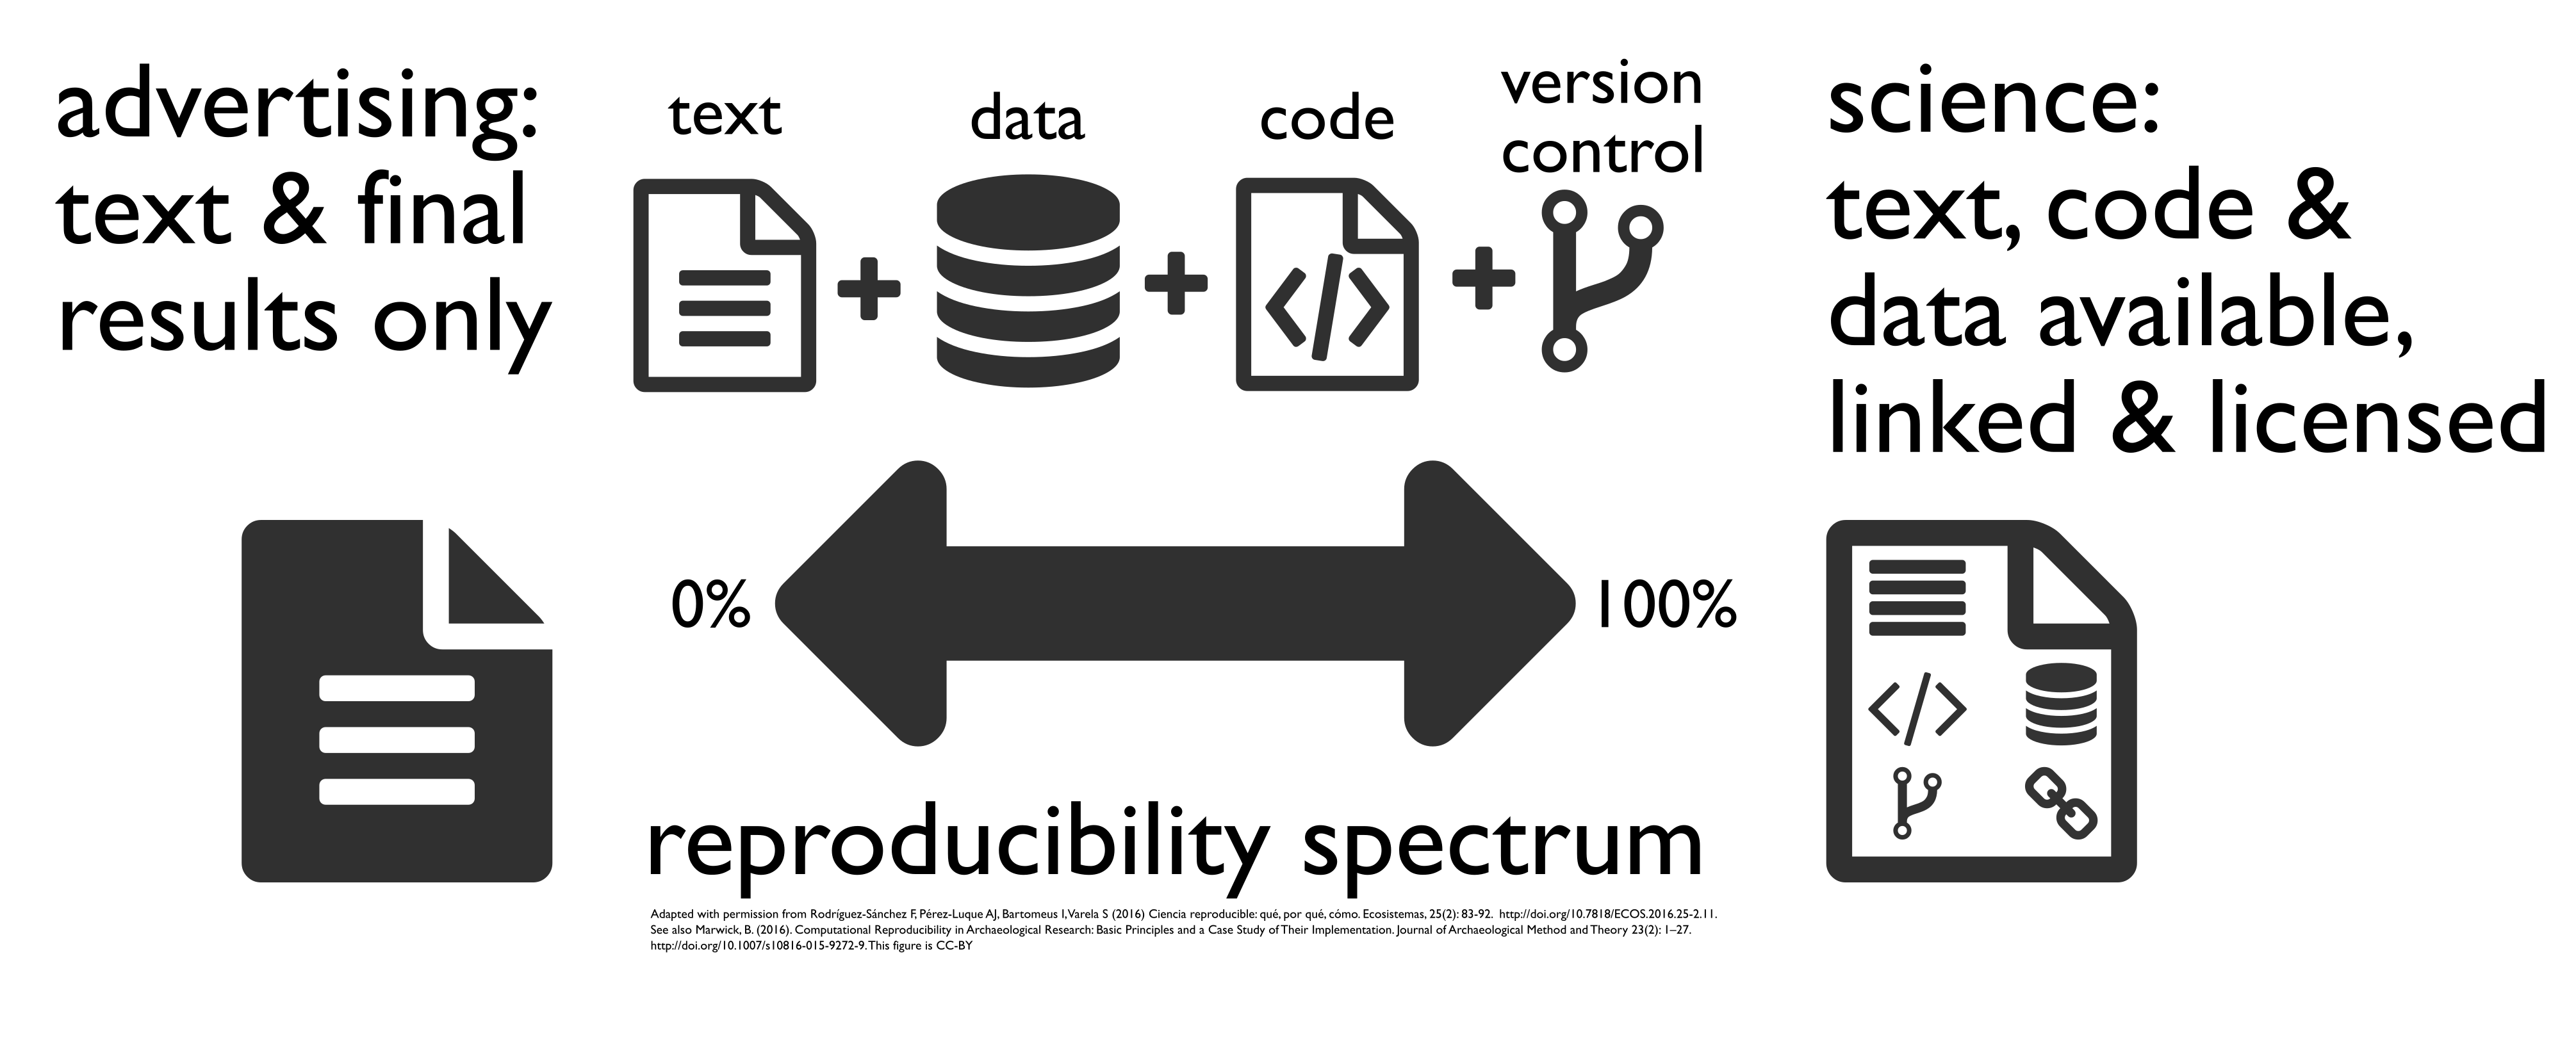
\includegraphics[width=1\linewidth]{figures/reproducible-research-spectrum} 

}

\caption{Reproducible research, Fig. 2 in {[}\protect\hyperlink{ref-marwick_2017}{9}{]}.}\label{fig:reproducible-research}
\end{figure}

\hypertarget{reproducibility-spectrum}{%
\subsection{Reproducibility Spectrum}\label{reproducibility-spectrum}}

Across the literature, researchers have identified a ``reproducibility spectrum'' ranging from the extreme, i.e.~publication only (advertising and marketing of the done work), to almost or even fully replicable research.
The work of Marwick et al.~{[}\protect\hyperlink{ref-marwick_2017}{9}{]} and Peng {[}\protect\hyperlink{ref-Peng1226}{11}{]} uses the analogy of a spectrum that can be mapped against the scoring of Vandewalle {[}\protect\hyperlink{ref-vandewalle_2009}{10}{]} describing the level of reproducibility on a 0 to 5 scale {[}\protect\hyperlink{ref-marwick_2017}{9}{]}.
In light of {[}\protect\hyperlink{ref-leek_2015}{12}{]}, this paper conceptualises reproducibility as the ``ability to recompute data analytic results given an observed dataset and knowledge of the data analysis pipeline'' and accordingly ``replicability of a study is the chance that an independent experiment targeting the same scientific question will produce a consistent result''.

With Fig. \ref{fig:reproducible-research} and the discussion in this section, this paper implements a fully reproducible workflow.
This is achieved by establishing this paper with open source software which allows to combine text, code, and visualisations.
The associated source text can also easily be read with a simple text editor/viewer. From that perspective, the text is fully inspectable.
This includes the majority of visualisations which are generated based on the data. Accordingly, the parameters and settings chosen can be validated by an independent researcher/analyst. Last but not least, the data for this paper is made available in conjunction with this text as Open Data. This also includes intermediate data artefacts which allows for the reproduction of the complete work or portions of it.
The conceptual approach and its building blocks will be presented in more detail in the next section.

\hypertarget{method-approach}{%
\section{Method / Approach}\label{method-approach}}

\hypertarget{conceptual-approach}{%
\subsection{Conceptual Approach}\label{conceptual-approach}}



\begin{figure}[hbt]

{\centering 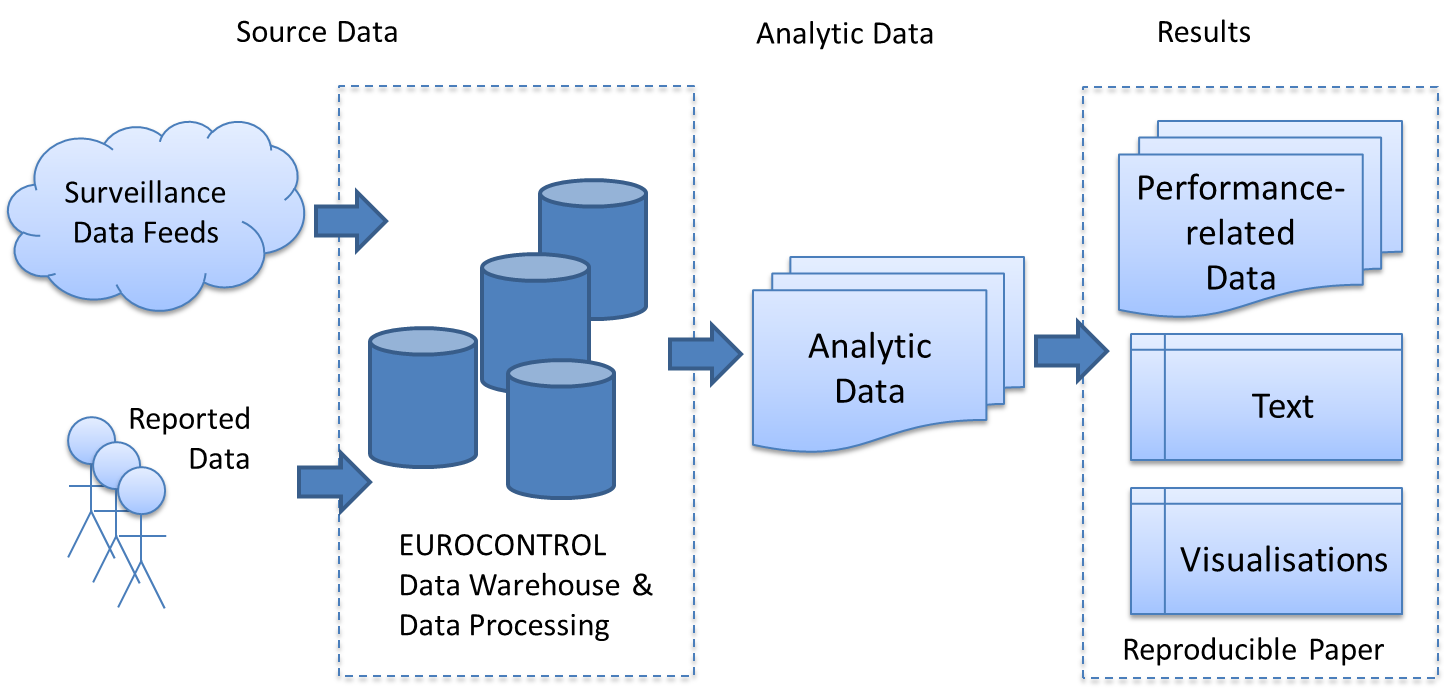
\includegraphics[width=1\linewidth]{figures/approach-stages} 

}

\caption{Conceptual approach to reproducibility by PRU.}\label{fig:concept-approach}
\end{figure}

This paper builds on the conceptual approach presented in Fig. \ref{fig:concept-approach} to implement replicable data analyses for performance monitoring and associated research.
On the data level this approach abstracts three levels of data:

\begin{itemize}
\tightlist
\item
  source data
\item
  analytical data
\item
  results (and performance related data)
\end{itemize}

The source data for this paper comprises the PRU Performance Reference Trajectory and operator reported data under the airport operator data flow. This study also uses some aeronautical information for the use case airports accessible through AIP or community maintained open data archives (e.g.~http://openaip.net, http://ourairports.com).
These data flows are processed and stored in the EUROCONTROL data warehouse.
The approach recognises that the full source data may or cannot be provided for a variety of reasons.
These include volume of the source data sets, technical constraints allowing access to the source data storage, and data sharing policies or use limitations.
For the latter cases, PRU promotes the sharing of a so-called representative sample.
The idea is that with the provision of the associated processing code, other researchers/practitioners are able to reconstruct a part of the analytic data - and subsequently part of the reported results - on the basis of the provided source data set.

Analytical data refers to the data sets established based on the aforementioned processing code.
An essential defining characteristic of analytic data is that it is the data basis on which the reported results can be produced.
The abstraction between source data and analytic data allows for the sharing of such data as limitations are typically only applicable to the source data. We follow the notion of {[}\protect\hyperlink{ref-marwick_2017}{9}{]} by referring to the provision of a representative sample of 8 days accompanying this paper as source data.

As depicted in Fig. \ref{fig:reproducible-research} the provision of the data, code, and text allows to move to the right part of the reproducibility spectrum, away from marketing and final results to credible, transparent, and challengeable analysis.
Accordingly, the results (or performance related data) level presents the final abstraction.

\hypertarget{toolset}{%
\subsection{Toolset}\label{toolset}}

This work builds on the RStudio tools for the R language {[}\protect\hyperlink{ref-rcoreteam_2018}{13}{]} including Git (and the web-based repository managers GitHub and GitLab) as underlying version control system.
The R language was originally developed within the statistical community supporting the task of statistical reporting by providing routines for the statistical computing and visualisation.
Being open source, the R community is actively engaging and sharing related software packages to enhance the core functionality.
Without limiting the impact of other packages, the development of knitr {[}\protect\hyperlink{ref-R-knitr}{14}{]} and RMarkdown {[}\protect\hyperlink{ref-xie2018}{15}{]}, ggplot {[}\protect\hyperlink{ref-wickham_2016}{16}{]} for visualisation, and the so-called tidyverse packages and RStudio IDE {[}\protect\hyperlink{ref-rstudioteam_2015}{17}{]} represent an open source ecosystem for data analysis.
A key feature for the implementation of the reproducibility paradigm is the fact that RMarkdown supports the combination of text, analytical code, and visualisations in a single document.
A minimal example of an RMarkdown document, a plain-text file with the conventional
extension \texttt{.Rmd} is shown below:

\footnotesize

\begin{Shaded}
\begin{Highlighting}[]
\OtherTok{---}
\FunctionTok{title:}\AttributeTok{ }\StringTok{"R Markdown example"}
\FunctionTok{author:}\AttributeTok{ }\StringTok{"John Doe"}
\FunctionTok{date:}\AttributeTok{ }\StringTok{"2019-02-17"}
\FunctionTok{output:}\AttributeTok{ html_document}
\OtherTok{---}
\end{Highlighting}
\end{Shaded}

\begin{Shaded}
\begin{Highlighting}[]
\NormalTok{Some math }
\NormalTok{$\textbackslash{}frac\{1\}\{N\} \textbackslash{}sum_\{i=1\}^N (x_i -\textbackslash{}mu)^2$,}
\NormalTok{followed by numbered list:}
  
\NormalTok{1. }\FloatTok{*italics* and **bold** text}
\FloatTok{1. then bullets}
\FloatTok{    - simple, eh?}

\NormalTok{and a code chunk:}

\BaseNTok{```\{r\}}
\BaseNTok{library(ggplot2)}
\BaseNTok{fit = lm(mpg ~ wt, data = mtcars)}
\BaseNTok{b   = coef(fit)}
\BaseNTok{ggplot(mtcars, aes(x = wt, y = mpg)) +}
\BaseNTok{  geom_point() + }
\BaseNTok{  geom_smooth(method = lm, se = TRUE)}
\BaseNTok{```}

\NormalTok{The slope of the regression is }\BaseNTok{`r b[1]`}\NormalTok{.}
\BaseNTok{```}
\end{Highlighting}
\end{Shaded}

\normalsize

There are three components of an R Markdown document: the metadata, the text and the code.
The metadata, written between the pair of three dashes \texttt{-\/-\/-}, helps in the production of
output document (title, type of document {[}web page, PDF, MS Word{]}, \ldots)
The text, which follows the metadata, is written using Markdown, a simplified formatting syntax
which can include prose and code.
There are two types of (computer) code:

\begin{itemize}
\item
  A code chunk starts with three backticks and \texttt{r} indicates the
  language name,\footnote{R Markdown supports 50 other computer languages.} and ends with
  three backticks.
\item
  An inline R code expression starts with backtick r and ends with a backtick.
\end{itemize}

Code portions are executed when the document is rendered.
Fig. \ref{fig:rmd-example} shows how the simple R Markdown example is rendered.



\begin{figure}[htb]

{\centering 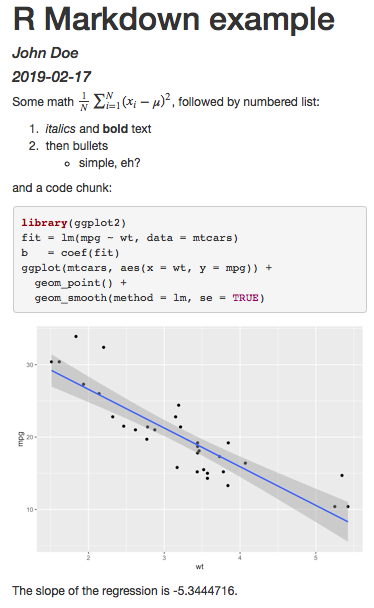
\includegraphics[width=1\linewidth]{figures/rmd-example} 

}

\caption{The output of a minimalist example of RMarkdown.}\label{fig:rmd-example}
\end{figure}

\hypertarget{capabilities-performance-reference-trajectory}{%
\subsection{Capabilities: Performance Reference Trajectory}\label{capabilities-performance-reference-trajectory}}

Throughout the recent year PRU developed the data analytical capabilities to fuse correlated position reports and ADSB surveillance data.
This work has been reported in {[}\protect\hyperlink{ref-koelle_open_2017}{8}{]} and {[}\protect\hyperlink{ref-spinielli_2018}{5}{]}. The idea is to establish a pan-European air situation picture openly available to researchers and practitioners.
Conceptually, the performance reference trajectory will be a key milestone in combatting the ``marketing myths.''
For example, operational improvements can be directly assessed by interested analysts as access to the Open Data enables the validation of the observable performance improvements. This allows for the application of commonly accepted methods and models to express performance benefits and ultimately challenge related publications on deployments and achieved improvements.

At the end of 2018 the initial development project phase was closed and PRU is now investigating options for deploying and maintaining the processing modules on a cloud platform.
The goal is to establish and operate the underlying data processing capabilities throughout 2019 and launch the regular provision of the performance reference trajectory as Open Data in 2020.

\hypertarget{results}{%
\section{Results}\label{results}}

\hypertarget{data-preparation}{%
\subsection{Data Preparation}\label{data-preparation}}

The raw data sources for the use cases of this paper have been processed by a pipeline of R scripts.
For example, the additional ASMA time indicator and the anticipated further breakdown of the arrival phase can be described by a set of transition points:

\begin{itemize}
\tightlist
\item
  segment I: entry into the ASMA area to entry into the holding/vectoring segment
\item
  segment II: holding/vectoring segment; for the use case reported holding stacks or point merge procedure
\item
  segment III: final approach alignment and approach
\end{itemize}



\begin{figure}[htb]

{\centering 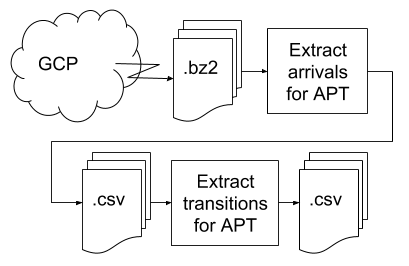
\includegraphics[width=1\linewidth]{figures/data-preparation-pipeline} 

}

\caption{Data preparation pipeline.}\label{fig:data-preparation-pipeline}
\end{figure}

Figure \ref{fig:data-preparation-pipeline} shows how the transition points
(40 NM, entry/exit from holding/point-merge area, landing) for the use case airports
have been extracted.
The following steps and scripts comprise {[}\protect\hyperlink{ref-performancereviewunit_2019}{18}{]}:

\begin{enumerate}
\def\labelenumi{\arabic{enumi}.}
\item
  the script \texttt{R/extract-arrivals.R} extracts arrivals to the \texttt{APT} airport and generates files with:

  \begin{itemize}
  \tightlist
  \item
    flight details
  \item
    arrivals' positions (\texttt{raw} and smoothed trajectories)
  \item
    (smoothed) arrivals' positions within 40 NM of the airport's reference position (ARP)
  \end{itemize}
\item
  the script \texttt{R/extract-transition-points.R} extracts transition points in the terminal area
  and generates a file containing per each flight:

  \begin{itemize}
  \tightlist
  \item
    the first point within 40 NM, \texttt{P40}
  \item
    the first and last point within the holding/point-merge area, \texttt{PHOLD}
  \item
    an estimated landing point, \texttt{PLAND}
  \end{itemize}
\end{enumerate}

This stage makes use of data extracted/extrapolated from the relevant AIP such
as ARP, runway name and threshold position/elevation, polygons for holding
stacks or point-merge areas. Specifically the polygons have been heuristically defined from the
point merge points in the AIP and enlarged by 2NM in order to cater for the spread of real flown
trajectories,
see the scripts \texttt{R/egll-data.R} and \texttt{R/eidw-data.R}.

Each transition position mentioned above consist of at least

\begin{itemize}
\tightlist
\item
  aircraft/flight info: ID, callsign, registration, ADEP/ADES, ICAO 24 bit address;
\item
  4D position: timestamp \(T\), longitude, latitude, altitude;
\item
  position info: flown distance \(D\) from aerodrome of departure (ADEP), sequence number,
  distance to ARP as a proxy of aerodrome of destination (ADES);
\item
  point info: sequence number, type of transition point {[}\texttt{P40}, \texttt{PHOLD}, \texttt{PLAND}{]}
\end{itemize}

These allow to calculate for each flight

\begin{itemize}
\tightlist
\item
  the time spent before the holding/point-merge area, \(T_{PHOLD|first} - T_{P40}\)
\item
  the distance flown before the holding/point-merge area,
  \(D_{PHOLD | first} - D_{P40}\)
\item
  the time spent within the holding/point-merge area, \(T_{PHOLD | last} - T_{PHOLD|first}\)
\item
  the distance flown within the holding/point-merge area,
  \(D_{PHOLD | last} - D_{PHOLD | first}\)
\item
  the time spent out of the holding/point-merge area till landing,
  \(T_{PLAND} - T_{PHOLD | last}\)
\item
  the distance flown out of the holding/point-merge area till landing,
  \(D_{PLAND} - D_{PHOLD | last}\)
\end{itemize}

\hypertarget{data-coverage}{%
\subsection{Data Coverage}\label{data-coverage}}

For this paper, a reproducible data set for the analysis of arrival management techniques at London Heathrow and Dublin airport have been extracted.
The data set comprises flights for the period of 1.-8. August 2017.
It can be inferred from the traffic mix at London Heathrow (major international hub) that only a limited subset of flights is not equipped with ADSB, while a slightly higher level of non-equipped flights is expected at Dublin (higher share of intra-European flights).



\begin{figure}[hbt]

{\centering \includegraphics[width=1\linewidth]{paper_files/figure-latex/coverage-egll-1} 

}

\caption{Number of arrivals in data sets, i.e.~1.-8. Aug 2017.}\label{fig:coverage-egll}
\end{figure}

Fig. \ref{fig:coverage-egll} shows the overlap of the data between the arrivals extracted from the airport operator data flow (APDF) and the reference trajectory (RTRJ) for London Heathrow (EGLL) and Dublin (EIDW).
For the time horizon of this paper, the coverage of the reference trajectory derived data is for Heathrow (EGLL) 100\% and for Dublin 97\%.

\hypertarget{replicate-asma-time-based}{%
\subsection{``replicate'' ASMA (time-based)}\label{replicate-asma-time-based}}

The additional time in the arrival sequencing and metering area (ASMA) is a globally recognised measure to assess flight efficiency during the arrival phase.
The ASMA metric calculates the additional time based on a reference time which is determined for a family of flights sharing similar characteristics.
For each flight \(i\) the additional ASMA time is

\[{add.~ASMA~time}_i = {actual~travel~time}_i - {reference~time}_i\]

The reference time \(i\) is determined for flights with similar arrival characteristics (c.f. \url{http://ansperformance.eu/references/definition/additional_asma_time.html}). These include 1.) the arrival entry sector at 40NM from the airport, 2.) the aircraft weight turbulence category and engine type, and 3.) the actual landing runway.
The reference times are built for a longer time horizon and extracted from the PRU data base as additional source data.



\begin{figure}[hbt]

{\centering \includegraphics[width=1\linewidth]{paper_files/figure-latex/ASMA-travel-egll-1} 

}

\caption{Distribution of actual ASMA travel times for EGLL (1.-8. Aug 2017).}\label{fig:ASMA-travel-egll}
\end{figure}

As an example, the distribution of the actual arrival transit times for arrivals into Heathrow (EGLL) are shown in Fig. \ref{fig:ASMA-travel-egll}. Heathrow operates holding stacks to tactically optimise the arrival throughput.
Dependent on the traffic situation, aircraft may experience longer holding times (i.e.~long tails of box plots in Fig. \ref{fig:ASMA-travel-egll}).

Fig. \ref{fig:ASMA-compare} compares the additional ASMA time extracted from the PRU performance dashboard, the trajectory based calculation with the dashboard derived reference time, and a 20-th percentile approach purely based on the trajectory data.



\begin{figure}[hbt]

{\centering \includegraphics[width=1\linewidth]{paper_files/figure-latex/ASMA-compare-1} 

}

\caption{Comparison of determined ASMA values, i.e.~1.-8. Aug 2017.}\label{fig:ASMA-compare}
\end{figure}

In Fig. \ref{fig:ASMA-compare}
APDFNM refers to the variant used for the EUROCONTROL Performance Review System. The reference time is build on the basis of a one-year sample. Applying this reference time to the trajectory based travel times (i.e.~TRJ-REF), there is a strong increase of the additional ASMA time for Heathrow (EGLL), while in the case of Dublin (EIDW) a reasonable decrease takes place. Calculating the additional ASMA time exclusively with the trajectory sample and applying a 20-th percentile approach (TRJ-20PCT), shows a significant drop in EGLL and a moderate increase at Dublin. The high variation for Heathrow shows that the additional ASMA time is strongly dependent on the time horizon.
The pure trajectory based measure - by definition - includes the effect of the operational concept (stack holdings) and distorts the measure. In the case of Dublin it can be argued that the TRJ-20PCT measure reflects the time based ASMA measure sufficiently.

\hypertarget{distance-based-asma}{%
\subsection{Distance-based ASMA}\label{distance-based-asma}}

Conceptually, measuring flight inefficiency in terms of flight time accounts for the airspace user perspective.
The previous section has also shown the high dependency of the time based measure on the sample size or reference time attribution.
Flight time is linked to engine time and accordingly, assuming manoeuvring for operational separation and sequencing reasons, fuel burn.
From a service provision perspective, efficiency relates to the capability to provide the least distance flown within the ASMA area.
In that respect, the data analytical capability to determine an associated additional distance flown metric addresses an open gap.



\begin{figure}[hbt]

{\centering \includegraphics[width=1\linewidth]{paper_files/figure-latex/ASMA-time-dist-1} 

}

\caption{Relationship travel time and distance flown, i.e.~1.-8. Aug 2017.}\label{fig:ASMA-time-dist}
\end{figure}

Fig. \ref{fig:ASMA-time-dist} shows the relationship between the actual distance flown and the actual time flown.
The variation of travel times is influenced by varying airspeeds or weather phenomena (e.g.~wind).
This paper applies a simple 15-th percentile approach to the distance flown per arrival sector, aircraft type/engine, and landing runway.
Tab. \ref{tab:tbl-asma-dist} lists the determined average additional distance at the study airports.
The total additional distance is determined as the aggregated sum of the differences in each segment
with 15-th percentile reference distance.

\begin{table}

\caption{\label{tab:tbl-asma-dist}Average additional distance flown (15-th pct)}
\centering
\begin{tabular}[t]{l|r|r|r}
\hline
AIRPORT & TOT\_ADD\_DIST & N\_ARRS & AVG\_ADD\_DIST\\
\hline
EGLL & 117014.9 & 5249 & 22.29\\
\hline
EIDW & 33081.9 & 2634 & 12.56\\
\hline
\end{tabular}
\end{table}

\hypertarget{arrival-management-practices}{%
\subsection{Arrival Management Practices}\label{arrival-management-practices}}

For an initial drill down, this paper uses arrival practices at London Heathrow and Dublin.
The approach to managing the arrival flow differs significantly between these airports.
Conceptually, London Heathrow employs the ``pressure on the runway'' concept with a focus on achieving and balancing a continuously high level of runway throughput utilisation.
This is accomplished by controlling the demand through 4 arrival stacks that allow for the tactical sequencing on the last portion of the approach.
Instead Dublin is one of the airports that pioneered the implementation of ``point merge''.
Point merge aims at replacing circular holdings by longitudinal holdings to establish the sequence based on predefined legs.



\begin{figure}[htb]

{\centering \includegraphics[width=1\linewidth]{paper_files/figure-latex/egll-trajectory-example-1} 

}

\caption{EGLL - long trajectory flown on 1. Aug 2017.}\label{fig:egll-trajectory-example}
\end{figure}



\begin{figure}[bht]

{\centering \includegraphics[width=1\linewidth]{paper_files/figure-latex/eidw-trajectory-example-1} 

}

\caption{EIDW - long trajectory flown on 1. Aug 2017.}\label{fig:eidw-trajectory-example}
\end{figure}

From a performance perspective it is therefore interesting to identify and measure the impact of the operational concept on the overall flight efficiency during the arrival phase of flight.

Fig. \ref{fig:egll-trajectory-example} and Fig. \ref{fig:eidw-trajectory-example} show examples
for long distances flown on 1. Aug 2017.
The trajectory data allows for the identification of the holdings and/or sequencing area so as
to separate the effect of the operational concepts.



\begin{figure}[H]

{\centering \includegraphics[width=1\linewidth]{paper_files/figure-latex/distance-flown-segment-1} 

}

\caption{Actual distances flown for each segment of the arrival phase (i.e.~EGLL, 1.-8. Aug 2017).}\label{fig:distance-flown-segment}
\end{figure}

Fig. \ref{fig:distance-flown-segment} depicts the flown distances per segment of the arrival phase.
In the case of London Heathrow the classical stack based holding can be seen in the significant variations of the actual distance flown per arrival direction.
Only limited sequencing takes place during the first segment (arrival within 40 NM and the stacks).



\begin{figure}[H]

{\centering \includegraphics[width=1\linewidth]{paper_files/figure-latex/distance-flown-segment-eidw-1} 

}

\caption{Actual distances flown for each segment of the arrival phase (i.e.~EIDW, 1.-8. Aug 2017).}\label{fig:distance-flown-segment-eidw}
\end{figure}

Fig. \ref{fig:distance-flown-segment-eidw} shows different footprint. It follows from the distribution of the initial approach segment that this portion is already used for sequencing and synchronisation by Dublin approach.
The middle segment shows a wider variation and less uniform distribution than the approach at London Heathrow.

Fig. \ref{fig:eidw-saturation-example} depicts the variation of the arrival segment throughput at Dublin (EIDW).
The median for every set of flights in the ASMA area versus flights landing is highlighted.
The behaviour is a classical saturation curve, i.e.~up to an arrival bunching of 10-11 flights per 20 min (30-33 flights per hour), the point merge procedure seems to be able to support the tactical absorption and sequencing.
It is noteworthy that the saturation curve falls for higher arrival throughputs. As no measurements for 12 through 14 landings had been made in the sample, this behaviour could be caused by the chosen time horizon.



\begin{figure}[hb]

{\centering \includegraphics[width=1\linewidth]{paper_files/figure-latex/eidw-saturation-example-1} 

}

\caption{EIDW - arrival throughput saturation (1.-8. Aug 2017).}\label{fig:eidw-saturation-example}
\end{figure}

\hypertarget{conclusions}{%
\section{Conclusions}\label{conclusions}}

The work reported establishes a fully reproducible paper for ANS performance in Europe.
It is the one of the first attempt to provide the artefacts that allow an independent researcher or professional to reproduce the results and verify upstream processing steps.
This paper follows up on previous work {[}\protect\hyperlink{ref-spinielli_2018}{5}{]}, {[}\protect\hyperlink{ref-koelle_open_2017}{8}{]}, {[}\protect\hyperlink{ref-spinielli_2017}{19}{]} and forms part of the roll-out of the performance reference trajectory by the PRU.
As such the paper demonstrates the feasibility to the approach, the data analytical capabilities and preprocessing, and the reporting via the R/RStudio ecosystem.
This represents an essential milestone moving towards the envisaged target environment.
However, further work is required to establish the reproducible environment for ANS Performance.

The move to open data for ANS Performance is a \emph{giant leap} in terms of transparency.
This will foster a new level of cooperation and discussion amongst researchers and professionals interested in this topic.
It removes the burden to acquire and preprocess large-scale surveillance data and associated aircraft data or aeronautical information.
The departure point for this development was to address the lack and hurdle of verifying results.
A further advantage is that novel applications, methods and algorithms (e.g.~machine learning), can be applied to a harmonised dataset.

The major application of the paper results will inform the performance reference trajectory project.
This goes in hand with the iterative move of the operational performance measures to trajectory derived data.
This can take on the form of quality assurance measures (e.g.~verifying the order of magnitude, complementing missing reported data), but also making the reference trajectory the primary means of data collection.
The latter will support the further development of the operational performance measures responding to the ICAO GANP.

This paper documents a key milestone in the project.
As such the future work will address the roll-out of the performance reference trajectory,
the establishment of the current performance reporting based on the trajectory (via \url{http://ansperformance.eu}, and setup of a network with interested researchers and professionals.

\hypertarget{references}{%
\section*{References}\label{references}}
\addcontentsline{toc}{section}{References}

\vspace{6pt}
\setlength{\parskip}{0pt}
\footnotesize
\setlength{\parindent}{0cm}

\hypertarget{refs}{}
\leavevmode\hypertarget{ref-kolata_2011}{}%
{[}1{]} G. Kolata, ``How a New Hope in Cancer Fell Apart,'' \emph{The New York Times: Health}, 07-Jul-2011.

\leavevmode\hypertarget{ref-ritchie_2012}{}%
{[}2{]} S. J. Ritchie, R. Wiseman, and C. C. French, ``Failing the future: Three unsuccessful attempts to replicate Bem's `Retroactive Facilitation of Recall'Effect,'' \emph{PloS one}, vol. 7, no. 3, p. e33423, 2012.

\leavevmode\hypertarget{ref-fraser_etal_2018}{}%
{[}3{]} H. Fraser, T. Parker, S. Nakagawa, A. Barnett, and F. Fidler, ``Questionable research practices in ecology and evolution,'' \emph{PloS one}, vol. 13, no. 7, p. e0200303, 2018.

\leavevmode\hypertarget{ref-fidler_wilcox_2018}{}%
{[}4{]} F. Fidler and J. Wilcox, ``Reproducibility of Scientific Results,'' in \emph{The Stanford Encyclopedia of Philosophy}, Winter 2018., E. N. Zalta, Ed. Metaphysics Research Lab, Stanford University, 2018.

\leavevmode\hypertarget{ref-spinielli_2018}{}%
{[}5{]} E. Spinielli, R. Koelle, K. Barker, and N. Korbey, ``Open Flight Trajectories for Reproducible ANS Performance Review,'' presented at the SESAR Innovation Days 2018, 2018, p. 8.

\leavevmode\hypertarget{ref-gandrud_2015}{}%
{[}6{]} C. Gandrud, \emph{Reproducible Research with R and R Studio, Second Edition (Chapman \& Hall/CRC The R Series)}. Routledge, 2015.

\leavevmode\hypertarget{ref-peteraldhous_2016}{}%
{[}7{]} C. S. Peter Aldhous, ``Spies in the Skies,'' \emph{See Maps Showing Where FBI Planes Are Watching From Above}, 06-Apr-2016. {[}Online{]}. Available: \url{https://www.buzzfeed.com/peteraldhous/spies-in-the-skies}.

\leavevmode\hypertarget{ref-koelle_open_2017}{}%
{[}8{]} R. Koelle, ``Open Source Software and Crowd Sourced Data for Operational Performance Analysis,'' presented at the USA/Europe ATM R\&D Seminar, 2017.

\leavevmode\hypertarget{ref-marwick_2017}{}%
{[}9{]} B. Marwick, ``Open Science in Archaeology,'' \emph{Open Science Framework}, Jan. 2017.

\leavevmode\hypertarget{ref-vandewalle_2009}{}%
{[}10{]} P. Vandewalle, J. Kovacevic, and M. Vetterli, ``Reproducible research in signal processing,'' \emph{IEEE Signal Processing Magazine}, vol. 26, no. 3, pp. 37--47, May 2009.

\leavevmode\hypertarget{ref-Peng1226}{}%
{[}11{]} R. D. Peng, ``Reproducible Research in Computational Science,'' \emph{Science}, vol. 334, no. 6060, pp. 1226--1227, 2011.

\leavevmode\hypertarget{ref-leek_2015}{}%
{[}12{]} J. T. Leek and R. D. Peng, ``Opinion: Reproducible research can still be wrong: Adopting a prevention approach,'' \emph{Proc Natl Acad Sci USA}, vol. 112, no. 6, p. 1645, Feb. 2015.

\leavevmode\hypertarget{ref-rcoreteam_2018}{}%
{[}13{]} R Core Team, \emph{R: A Language and Environment for Statistical Computing}. Vienna, Austria: R Foundation for Statistical Computing, 2018.

\leavevmode\hypertarget{ref-R-knitr}{}%
{[}14{]} Y. Xie, \emph{Knitr: A General-Purpose Package for Dynamic Report Generation in R}. 2018.

\leavevmode\hypertarget{ref-xie2018}{}%
{[}15{]} Y. Xie, J. J. Allaire, and G. Grolemund, \emph{R Markdown: The Definitive Guide}. Boca Raton, Florida: Chapman and Hall/CRC, 2018.

\leavevmode\hypertarget{ref-wickham_2016}{}%
{[}16{]} H. Wickham, \emph{Ggplot2: Elegant Graphics for Data Analysis}. Springer-Verlag New York, 2016.

\leavevmode\hypertarget{ref-rstudioteam_2015}{}%
{[}17{]} RStudio Team, \emph{RStudio: Integrated Development Environment for R}. Boston, MA: RStudio, Inc., 2015.

\leavevmode\hypertarget{ref-performancereviewunit_2019}{}%
{[}18{]} Performance Review Unit, ``Reference trajectories for Performance Review of European ANS,'' 2019. {[}Online{]}. Available: \url{https://doi.org/10.5281/zenodo.2566844}.

\leavevmode\hypertarget{ref-spinielli_2017}{}%
{[}19{]} E. Spinielli, R. Koelle, M. Zanin, and S. Belkoura, ``Initial Implementation of Reference Trajectories for Performance Review,'' \emph{SESAR Innovation Days}, no. 7, p. 8, 2017.

\end{document}


